\section{Lock bits e clock}
Il clock usato dal uC in genere è esterno, ma il modello che stiamo analizzando ha al suo interno varie sorgenti di clock che possono essere utilizzate se non si vuole usare una fonte esterna.
Le tensioni di operatività sono:
\begin{itemize}
    \item 2.7 - 3.6V per ATMega32L (3.3V $\pm$ 10\%)
    \item 4.5 - 5.5V per ATMega32 (5V $\pm$ 10\%)
\end{itemize}
quindi il clock deve essere un' onda quadra che vada da 0V a Vdd con duty cycle del 50\%.
Per programmare il clock interno si deve ricorrere ai \emph{fuse} interni.

Il concetto di fuse (fusibile) era inizialmente utilizzato all' interno delle PROM, ogni singola cella era un fusibile, in fase di programmazione si faceva saltare o meno tramite apposite tensioni, questo metodo tuttavia non era molto reliable in quanto i microcrateri causati da queste detonazioni potevano richiudersi grazie ai detriti e quindi riprendere a condurre.
In seguito si è passati agli antifusibili cioè dei condensatori che di norma non conducono, quando gli si fa passare una corrente adeguata invece il dielettrico diventa una giunzione permanente.

In fine all' interno del uC vi è un' altra memoria flash a parte, detta \emph{lockbits}, che contiene dei bit utilizzati per la configurazione dell' hardware.

\subsection{Lock bits}

\subsubsection{Lock bit byte}
Sono bit usati per impedire la lettura della flash e quindi dumpare il firmware contenuto nel uC, ce n'è uno anche per impedire la riprogrammazione.

\subsubsection{Bit clock option}
E' il quarto bit del fuse high byte e si usa per indicare quale modalità operativa deve usare l' oscillatore amplificatore.

\subsubsection{Clock select}
Sono i bit 3, 2, 1, 0 del fuse low byte e si usano per indicare quale sorgente di clock il uC deve usare.

\subsubsection{Start-up time}
Sono i bit 5, 4 del fuse low byte, sono usati per indicare lo startup time del clock. 

\subsubsection{Signature bytes}
Sono byte impressi in fabbrica per indicare quale modello di uC si sta utilizzando.
Sono utilizzati dall' hardware programmatore per rilevare quale hardware si sta per andare a programmare.

\subsubsection{Calibration bytes}
Sono byte utilizzti per regolare la velocità del clock in quanto il clock non è sempre preciso.
Si può tuttavia calibrare in base alle condizioni di utilizzo.
Dalla fabbrica escono programmati in maniera che il clock sia vicino a quanto dichiarato in condizioni di laboratorio, se si lavora lontano dalle condizioni di laboratorio conviene rieseguire la calibrazione.

\subsection{Clock}
Abbiamo 5 sorgenti di clock tra le quali scegliere, queste 5 sorgenti sono inserite all' interno di un multiplexer e tramite i bit clock select si sceglie quale uscita commutare.

\begin{table}[ht!]
    \centering
    \begin{tabular}{p{0.2\linewidth} | p{0.6\linewidth}}
        CKSEL3..0 & Descrizione \\
        \hline
        1111 - 1010 &  Oscillatre ceramico/quarzo esterno ad alte frequenze \\
        1001 & Cristallo esterno a basse frequenze \\
        1000 - 0101 & Oscillatore RC esterno si sceglie la frequenza \\
        0100 - 0001 & Oscillatore RC interno calibrato, si sceglie la capacità \\
        0000 & Clock esterno \\
    \end{tabular}
\end{table}
Di default si ha 0001.

\subsubsection{Circuito generale}
Il circuito generale del clock è:
\begin{figure}[H]
    \centering
    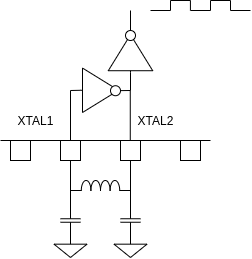
\includegraphics[width=200px]{images/17_Clock/basic_clock_generator.png}
\end{figure}
Tra i pin XTAL1 ed XTAL2 abbiamo un amplificatore invertente, XTAL1 è a alta impedenza mentre XTAL2 è a bassa impedenza.
Nella funzione di trasferimento del circuito abbiamo 3 poli in quanto abbiamo 3 elementi reattivi, quindi esiste una sola frequenza tale che la fase tra i due pin è 180°.
\begin{figure}[H]
    \centering
    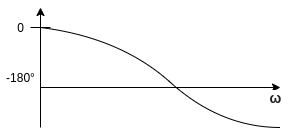
\includegraphics[width=300px]{images/17_Clock/frequency_response.png}
\end{figure}
Solo per la frequenza nella quale si ha l' intersezione il circuito è un oscillatore perfetto.
La frequenza alla quale si trova questa intersezione è fortemente dipendente dalla posizione dei poli, quindi dai valori degli elementi reattivi.

Per essere più precisi spesso si utilizza un cristallo risuonatore che ha una oscillazione ad una frequenza ben precisa: di solito si usa un cristallo di quarzo che essendo un elemento circuitale piezoelettrico ha una vibrazione meccanica facilmente prevedibile in base alla massa del cristallo.
\begin{figure}[H]
    \centering
    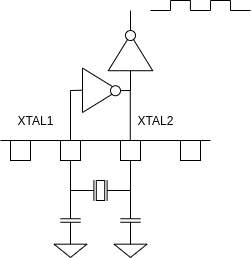
\includegraphics[width=200px]{images/17_Clock/crystal_oscillator.png}
\end{figure}
Il suo circuito equivalente è:
\begin{figure}[H]
    \centering
    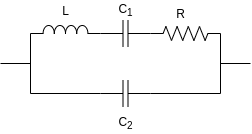
\includegraphics[width=200px]{images/17_Clock/equivalent_circuit.png}
\end{figure}
in cui:
\begin{itemize}
    \item $L$: è dovuto alla massa del cristallo, è come una molla
    \item $C_1$: è dovuto alla rigidità meccanica del pezzetto di cristallo
    \item $C_2$: dovuto alla capacità delle armature che ingabbiano il cristallo. $C_2 \sim 100C_1$
    \item $R$: corrisponde all' attrito che porterebbe a stoppare l' oscillazione
\end{itemize}
Approssimiamo l' impedenza del parallelo (trascuriamo la resistenza perché molto piccola):
\begin{itemize}
    \item in 0 abbiamo solo la capacità quindi abbiamo impedenza negativa
    \item la serie $L$ e $C_1$ si annulla quando sono uguali ed opposti, l' altro ramo è in parallelo quindi rimane zero, questa frequenza è $\omega_s$
    \item posso avere risonanza anche quando i due rami si annullano, questa frequenza la chiamiamo $\omega_p$
    \item sappiamo che $\omega_s < \omega_p$ e che in $\omega_p$ l' impedenza è infinita
\end{itemize}
\begin{figure}[H]
    \centering
    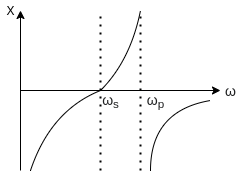
\includegraphics[width=200px]{images/17_Clock/impedence.png}
\end{figure}
Possiamo quindi dire:
\begin{itemize}
    \item $\omega < \omega_s$: è un condensatore
    \item $\omega > \omega_p$: è un condensatore
    \item $\omega_s < \omega < \omega_p$: è un induttore
\end{itemize}
Quindi all' interno di quel range il cristallo si comporta come un induttore, il range è tuttavia molto ristretto e molto preciso:
$$ |\omega_p - \omega_s| < 10^{-4} $$
Per esempio se: $\omega_s = 1$MHz allora $\omega_p = 1,0001$MHz quindi $\Delta{f} = 100$Hz è il range induttivo.
Abbiamo quindi un risuonatore con finestra di $100$Hz.

NB: i quarzi più economici di solito hanno $\Delta{f} = 30$Hz mentre quelli più costosi $\Delta{f} = 5$Hz.

Se volessi fare di meglio potrei utilizzare un cristallo termostatato cioè un cristallo a temperatura controllata e costante ottenuto usando una resistenza per mantenere la temperatura circa costante.


\subsubsection{Oscillatore a rilassamento}
Un altro oscillatore che possiamo utilizzare è quello a rilassamento:
\begin{figure}[H]
    \centering
    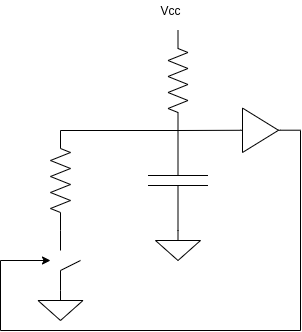
\includegraphics[width=150px]{images/17_Clock/relaxation_oscillator.png}
\end{figure}
Quando il condensatore si carica, lo facciamo caricare fino ai $\frac{2}{3}$, successivamente lo facciamo scaricare fino ai $\frac{1}{3}$ e così via ciclicamente.
\begin{figure}[H]
    \centering
    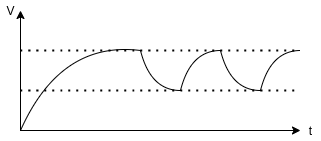
\includegraphics[width=200px]{images/17_Clock/relaxation_time_graph.png}
\end{figure}
La frequenza è esprimibile nella forma:
$$ f = \frac{\alpha}{RC} $$
ed è fortemente dipendente dalla precisione con la quale si scelgono i valori delle componenti, in genere va attorno al 1-3\%.

Nel nostro uC possiamo usare l'amplificatore che già c'è aggiungendo giusto un paio di componenti esterne:
\begin{figure}[H]
    \centering
    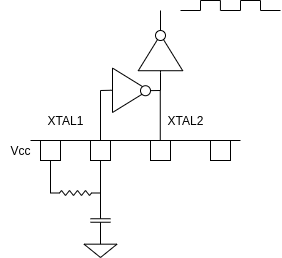
\includegraphics[width=200px]{images/17_Clock/relaxation_in_uC.png}
\end{figure}

Un' altra possibilità è quella di utilizzare la rete RC interna del uC.

\subsubsection{Clock esterno}
Possiamo usare un clock esterno direttamente inserito in XTAL1:
\begin{figure}[H]
    \centering
    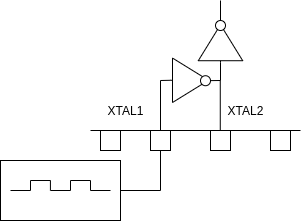
\includegraphics[width=200px]{images/17_Clock/external_clock.png}
\end{figure}
Questo è tipico dei sistemi a 2 uC in cui uno ha un generatore di clock con cristallo e l'altro usa il clock generato dal primo per funzionare:
\begin{figure}[H]
    \centering
    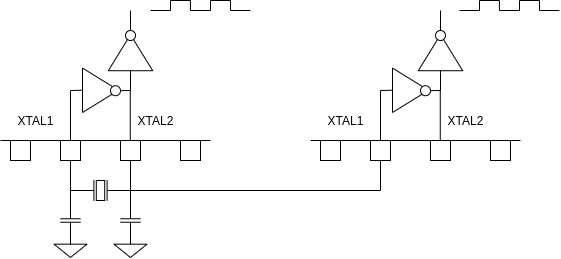
\includegraphics[width=300px]{images/17_Clock/back_to_back.png}
\end{figure}


